%%%%%%%%%%%%%%%%%%%%%%%%%%%%%%%%%%%%%%%%%
% University Assignment Title Page 
% LaTeX Template
% Version 1.0 (27/12/12)
%
% This template has been downloaded from:
% http://www.LaTeXTemplates.com
%
% Original author:
% WikiBooks (http://en.wikibooks.org/wiki/LaTeX/Title_Creation)
%
% License:
% CC BY-NC-SA 3.0 (http://creativecommons.org/licenses/by-nc-sa/3.0/)
% 
% Instructions for using this template:
% This title page is capable of being compiled as is. This is not useful for 
% including it in another document. To do this, you have two options: 
%
% 1) Copy/paste everything between \begin{document} and \end{document} 
% starting at \begin{titlepage} and paste this into another LaTeX file where you 
% want your title page.
% OR
% 2) Remove everything outside the \begin{titlepage} and \end{titlepage} and 
% move this file to the same directory as the LaTeX file you wish to add it to. 
% Then add %%%%%%%%%%%%%%%%%%%%%%%%%%%%%%%%%%%%%%%%%
% University Assignment Title Page 
% LaTeX Template
% Version 1.0 (27/12/12)
%
% This template has been downloaded from:
% http://www.LaTeXTemplates.com
%
% Original author:
% WikiBooks (http://en.wikibooks.org/wiki/LaTeX/Title_Creation)
%
% License:
% CC BY-NC-SA 3.0 (http://creativecommons.org/licenses/by-nc-sa/3.0/)
% 
% Instructions for using this template:
% This title page is capable of being compiled as is. This is not useful for 
% including it in another document. To do this, you have two options: 
%
% 1) Copy/paste everything between \begin{document} and \end{document} 
% starting at \begin{titlepage} and paste this into another LaTeX file where you 
% want your title page.
% OR
% 2) Remove everything outside the \begin{titlepage} and \end{titlepage} and 
% move this file to the same directory as the LaTeX file you wish to add it to. 
% Then add %%%%%%%%%%%%%%%%%%%%%%%%%%%%%%%%%%%%%%%%%
% University Assignment Title Page 
% LaTeX Template
% Version 1.0 (27/12/12)
%
% This template has been downloaded from:
% http://www.LaTeXTemplates.com
%
% Original author:
% WikiBooks (http://en.wikibooks.org/wiki/LaTeX/Title_Creation)
%
% License:
% CC BY-NC-SA 3.0 (http://creativecommons.org/licenses/by-nc-sa/3.0/)
% 
% Instructions for using this template:
% This title page is capable of being compiled as is. This is not useful for 
% including it in another document. To do this, you have two options: 
%
% 1) Copy/paste everything between \begin{document} and \end{document} 
% starting at \begin{titlepage} and paste this into another LaTeX file where you 
% want your title page.
% OR
% 2) Remove everything outside the \begin{titlepage} and \end{titlepage} and 
% move this file to the same directory as the LaTeX file you wish to add it to. 
% Then add %%%%%%%%%%%%%%%%%%%%%%%%%%%%%%%%%%%%%%%%%
% University Assignment Title Page 
% LaTeX Template
% Version 1.0 (27/12/12)
%
% This template has been downloaded from:
% http://www.LaTeXTemplates.com
%
% Original author:
% WikiBooks (http://en.wikibooks.org/wiki/LaTeX/Title_Creation)
%
% License:
% CC BY-NC-SA 3.0 (http://creativecommons.org/licenses/by-nc-sa/3.0/)
% 
% Instructions for using this template:
% This title page is capable of being compiled as is. This is not useful for 
% including it in another document. To do this, you have two options: 
%
% 1) Copy/paste everything between \begin{document} and \end{document} 
% starting at \begin{titlepage} and paste this into another LaTeX file where you 
% want your title page.
% OR
% 2) Remove everything outside the \begin{titlepage} and \end{titlepage} and 
% move this file to the same directory as the LaTeX file you wish to add it to. 
% Then add \input{./title_page_1.tex} to your LaTeX file where you want your
% title page.
%
%%%%%%%%%%%%%%%%%%%%%%%%%%%%%%%%%%%%%%%%%
%\title{Title page with logo}
%----------------------------------------------------------------------------------------
%	PACKAGES AND OTHER DOCUMENT CONFIGURATIONS
%----------------------------------------------------------------------------------------

\documentclass[12pt]{article}
\usepackage[english]{babel}
\usepackage[utf8x]{inputenc}
\usepackage{amsmath}
\usepackage{graphicx}
\usepackage[colorinlistoftodos]{todonotes}

\begin{document}

\begin{titlepage}

\newcommand{\HRule}{\rule{\linewidth}{0.5mm}} % Defines a new command for the horizontal lines, change thickness here

\center % Center everything on the page
 
%----------------------------------------------------------------------------------------
%	HEADING SECTIONS
%----------------------------------------------------------------------------------------

\textsc{\LARGE Politenico di Milano}\\[1.5cm] % Name of your university/college
\textsc{\Large Dipartimento Elettronica, Informazione e Bioingegneria}\\[0.5cm] % Major heading such as course name
\textsc{\large HEAPLab Project Report}\\[0.5cm] % Minor heading such as course title

%----------------------------------------------------------------------------------------
%	TITLE SECTION
%----------------------------------------------------------------------------------------

\HRule \\[0.4cm]
{ \huge \bfseries Title}\\[0.4cm] % Title of your document
\HRule \\[1.5cm]
 
%----------------------------------------------------------------------------------------
%	AUTHOR SECTION
%----------------------------------------------------------------------------------------

\begin{minipage}{0.4\textwidth}
\begin{flushleft} \large
\emph{Author:}\\
John \textsc{Smith} % Your name
\end{flushleft}
\end{minipage}
~
\begin{minipage}{0.4\textwidth}
\begin{flushright} \large
\emph{Supervisor:} \\
Dr. Giusppe \textsc{Massari} % Supervisor's Name
\end{flushright}
\end{minipage}\\[2cm]

% If you don't want a supervisor, uncomment the two lines below and remove the section above
%\Large \emph{Author:}\\
%John \textsc{Smith}\\[3cm] % Your name

%----------------------------------------------------------------------------------------
%	DATE SECTION
%----------------------------------------------------------------------------------------

{\large \today}\\[2cm] % Date, change the \today to a set date if you want to be precise

%----------------------------------------------------------------------------------------
%	LOGO SECTION
%----------------------------------------------------------------------------------------


\includegraphics[width=100pt]{heaplogo.pdf}\\[1cm] % Include a department/university logo - this will require the graphicx package
 
%----------------------------------------------------------------------------------------

\vfill % Fill the rest of the page with whitespace

\end{titlepage}




\begin{abstract}
Your abstract. - Summarize your work.
\end{abstract}

\section{Introduction}

Your introduction goes here! Some examples of commonly used commands and features are listed below, to help you get started.

If you have a question, please use the support box in the bottom right of the screen to get in touch. 


\section{Design and Implementation}

\section{Experimental Results}

\section{Conclusions}


\section{Some \LaTeX{} Examples}
\label{sec:examples}

\subsection{Sections}

Use section and subsection commands to organize your document. \LaTeX{} handles all the formatting and numbering automatically. Use ref and label commands for cross-references.

\subsection{Comments}

Comments can be added to the margins of the document using the \todo{Here's a comment in the margin!} todo command, as shown in the example on the right. You can also add inline comments too:

\todo[inline, color=green!40]{This is an inline comment.}

\subsection{Tables and Figures}

Use the table and tabular commands for basic tables --- see Table~\ref{tab:widgets}, for example. You can upload a figure (JPEG, PNG or PDF) using the files menu. To include it in your document, use the includegraphics command as in the code for Figure~\ref{fig:frog} below.

% Commands to include a figure:
\begin{figure}
\centering
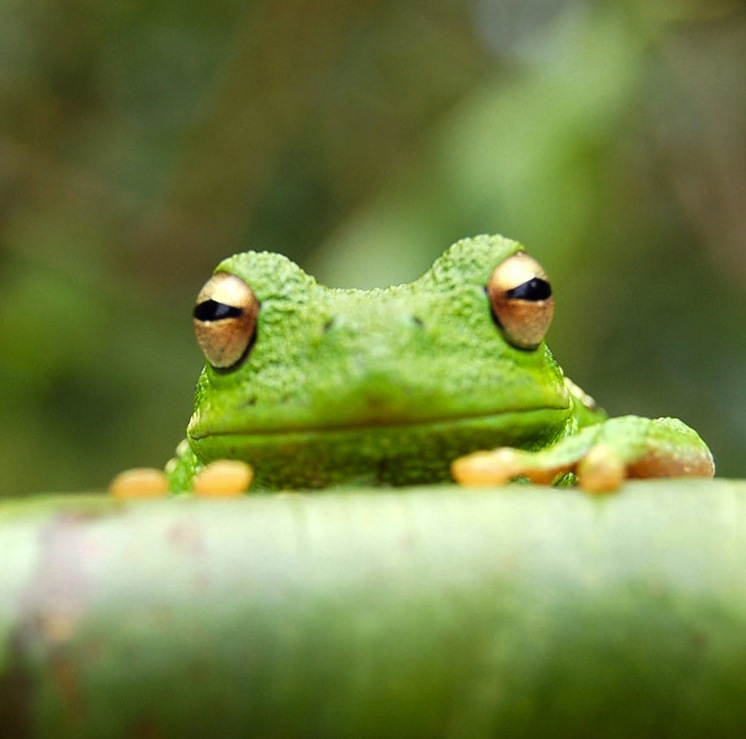
\includegraphics[width=0.5\textwidth]{frog.jpg}
\caption{\label{fig:frog}This is a figure caption.}
\end{figure}

\begin{table}
\centering
\begin{tabular}{l|r}
Item & Quantity \\\hline
Widgets & 42 \\
Gadgets & 13
\end{tabular}
\caption{\label{tab:widgets}An example table.}
\end{table}

\subsection{Mathematics}

\LaTeX{} is great at typesetting mathematics. Let $X_1, X_2, \ldots, X_n$ be a sequence of independent and identically distributed random variables with $\text{E}[X_i] = \mu$ and $\text{Var}[X_i] = \sigma^2 < \infty$, and let
$$S_n = \frac{X_1 + X_2 + \cdots + X_n}{n}
      = \frac{1}{n}\sum_{i}^{n} X_i$$
denote their mean. Then as $n$ approaches infinity, the random variables $\sqrt{n}(S_n - \mu)$ converge in distribution to a normal $\mathcal{N}(0, \sigma^2)$.

\subsection{Lists}

You can make lists with automatic numbering \dots

\begin{enumerate}
\item Like this,
\item and like this.
\end{enumerate}
\dots or bullet points \dots
\begin{itemize}
\item Like this,
\item and like this.
\end{itemize}

We hope you find write\LaTeX\ useful, and please let us know if you have any feedback using the help menu above.

\end{document} to your LaTeX file where you want your
% title page.
%
%%%%%%%%%%%%%%%%%%%%%%%%%%%%%%%%%%%%%%%%%
%\title{Title page with logo}
%----------------------------------------------------------------------------------------
%	PACKAGES AND OTHER DOCUMENT CONFIGURATIONS
%----------------------------------------------------------------------------------------

\documentclass[12pt]{article}
\usepackage[english]{babel}
\usepackage[utf8x]{inputenc}
\usepackage{amsmath}
\usepackage{graphicx}
\usepackage[colorinlistoftodos]{todonotes}

\begin{document}

\begin{titlepage}

\newcommand{\HRule}{\rule{\linewidth}{0.5mm}} % Defines a new command for the horizontal lines, change thickness here

\center % Center everything on the page
 
%----------------------------------------------------------------------------------------
%	HEADING SECTIONS
%----------------------------------------------------------------------------------------

\textsc{\LARGE Politenico di Milano}\\[1.5cm] % Name of your university/college
\textsc{\Large Dipartimento Elettronica, Informazione e Bioingegneria}\\[0.5cm] % Major heading such as course name
\textsc{\large HEAPLab Project Report}\\[0.5cm] % Minor heading such as course title

%----------------------------------------------------------------------------------------
%	TITLE SECTION
%----------------------------------------------------------------------------------------

\HRule \\[0.4cm]
{ \huge \bfseries Title}\\[0.4cm] % Title of your document
\HRule \\[1.5cm]
 
%----------------------------------------------------------------------------------------
%	AUTHOR SECTION
%----------------------------------------------------------------------------------------

\begin{minipage}{0.4\textwidth}
\begin{flushleft} \large
\emph{Author:}\\
John \textsc{Smith} % Your name
\end{flushleft}
\end{minipage}
~
\begin{minipage}{0.4\textwidth}
\begin{flushright} \large
\emph{Supervisor:} \\
Dr. Giusppe \textsc{Massari} % Supervisor's Name
\end{flushright}
\end{minipage}\\[2cm]

% If you don't want a supervisor, uncomment the two lines below and remove the section above
%\Large \emph{Author:}\\
%John \textsc{Smith}\\[3cm] % Your name

%----------------------------------------------------------------------------------------
%	DATE SECTION
%----------------------------------------------------------------------------------------

{\large \today}\\[2cm] % Date, change the \today to a set date if you want to be precise

%----------------------------------------------------------------------------------------
%	LOGO SECTION
%----------------------------------------------------------------------------------------


\includegraphics[width=100pt]{heaplogo.pdf}\\[1cm] % Include a department/university logo - this will require the graphicx package
 
%----------------------------------------------------------------------------------------

\vfill % Fill the rest of the page with whitespace

\end{titlepage}




\begin{abstract}
Your abstract. - Summarize your work.
\end{abstract}

\section{Introduction}

Your introduction goes here! Some examples of commonly used commands and features are listed below, to help you get started.

If you have a question, please use the support box in the bottom right of the screen to get in touch. 


\section{Design and Implementation}

\section{Experimental Results}

\section{Conclusions}


\section{Some \LaTeX{} Examples}
\label{sec:examples}

\subsection{Sections}

Use section and subsection commands to organize your document. \LaTeX{} handles all the formatting and numbering automatically. Use ref and label commands for cross-references.

\subsection{Comments}

Comments can be added to the margins of the document using the \todo{Here's a comment in the margin!} todo command, as shown in the example on the right. You can also add inline comments too:

\todo[inline, color=green!40]{This is an inline comment.}

\subsection{Tables and Figures}

Use the table and tabular commands for basic tables --- see Table~\ref{tab:widgets}, for example. You can upload a figure (JPEG, PNG or PDF) using the files menu. To include it in your document, use the includegraphics command as in the code for Figure~\ref{fig:frog} below.

% Commands to include a figure:
\begin{figure}
\centering
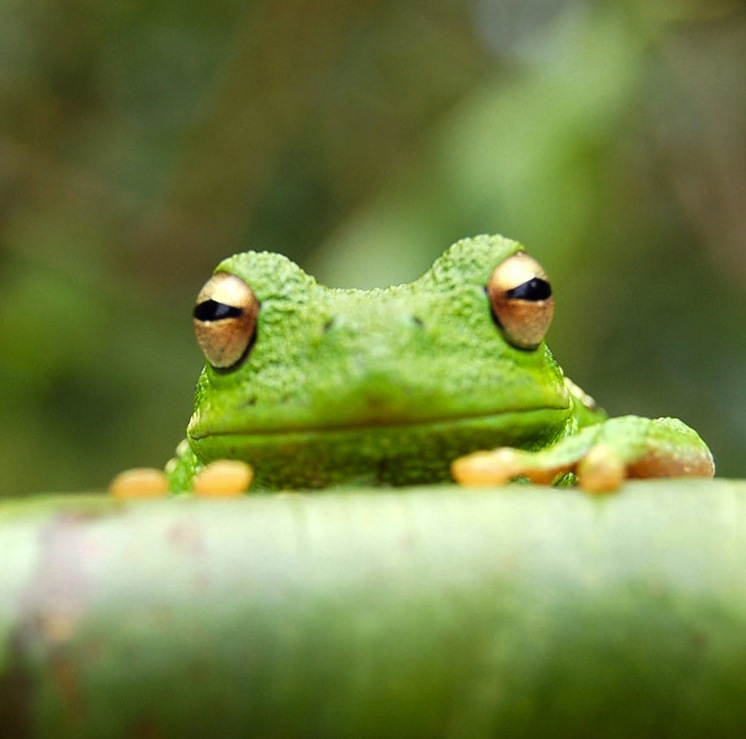
\includegraphics[width=0.5\textwidth]{frog.jpg}
\caption{\label{fig:frog}This is a figure caption.}
\end{figure}

\begin{table}
\centering
\begin{tabular}{l|r}
Item & Quantity \\\hline
Widgets & 42 \\
Gadgets & 13
\end{tabular}
\caption{\label{tab:widgets}An example table.}
\end{table}

\subsection{Mathematics}

\LaTeX{} is great at typesetting mathematics. Let $X_1, X_2, \ldots, X_n$ be a sequence of independent and identically distributed random variables with $\text{E}[X_i] = \mu$ and $\text{Var}[X_i] = \sigma^2 < \infty$, and let
$$S_n = \frac{X_1 + X_2 + \cdots + X_n}{n}
      = \frac{1}{n}\sum_{i}^{n} X_i$$
denote their mean. Then as $n$ approaches infinity, the random variables $\sqrt{n}(S_n - \mu)$ converge in distribution to a normal $\mathcal{N}(0, \sigma^2)$.

\subsection{Lists}

You can make lists with automatic numbering \dots

\begin{enumerate}
\item Like this,
\item and like this.
\end{enumerate}
\dots or bullet points \dots
\begin{itemize}
\item Like this,
\item and like this.
\end{itemize}

We hope you find write\LaTeX\ useful, and please let us know if you have any feedback using the help menu above.

\end{document} to your LaTeX file where you want your
% title page.
%
%%%%%%%%%%%%%%%%%%%%%%%%%%%%%%%%%%%%%%%%%
%\title{Title page with logo}
%----------------------------------------------------------------------------------------
%	PACKAGES AND OTHER DOCUMENT CONFIGURATIONS
%----------------------------------------------------------------------------------------

\documentclass[12pt]{article}
\usepackage[english]{babel}
\usepackage[utf8x]{inputenc}
\usepackage{amsmath}
\usepackage{graphicx}
\usepackage[colorinlistoftodos]{todonotes}

\begin{document}

\begin{titlepage}

\newcommand{\HRule}{\rule{\linewidth}{0.5mm}} % Defines a new command for the horizontal lines, change thickness here

\center % Center everything on the page
 
%----------------------------------------------------------------------------------------
%	HEADING SECTIONS
%----------------------------------------------------------------------------------------

\textsc{\LARGE Politenico di Milano}\\[1.5cm] % Name of your university/college
\textsc{\Large Dipartimento Elettronica, Informazione e Bioingegneria}\\[0.5cm] % Major heading such as course name
\textsc{\large HEAPLab Project Report}\\[0.5cm] % Minor heading such as course title

%----------------------------------------------------------------------------------------
%	TITLE SECTION
%----------------------------------------------------------------------------------------

\HRule \\[0.4cm]
{ \huge \bfseries Title}\\[0.4cm] % Title of your document
\HRule \\[1.5cm]
 
%----------------------------------------------------------------------------------------
%	AUTHOR SECTION
%----------------------------------------------------------------------------------------

\begin{minipage}{0.4\textwidth}
\begin{flushleft} \large
\emph{Author:}\\
John \textsc{Smith} % Your name
\end{flushleft}
\end{minipage}
~
\begin{minipage}{0.4\textwidth}
\begin{flushright} \large
\emph{Supervisor:} \\
Dr. Giusppe \textsc{Massari} % Supervisor's Name
\end{flushright}
\end{minipage}\\[2cm]

% If you don't want a supervisor, uncomment the two lines below and remove the section above
%\Large \emph{Author:}\\
%John \textsc{Smith}\\[3cm] % Your name

%----------------------------------------------------------------------------------------
%	DATE SECTION
%----------------------------------------------------------------------------------------

{\large \today}\\[2cm] % Date, change the \today to a set date if you want to be precise

%----------------------------------------------------------------------------------------
%	LOGO SECTION
%----------------------------------------------------------------------------------------


\includegraphics[width=100pt]{heaplogo.pdf}\\[1cm] % Include a department/university logo - this will require the graphicx package
 
%----------------------------------------------------------------------------------------

\vfill % Fill the rest of the page with whitespace

\end{titlepage}




\begin{abstract}
Your abstract. - Summarize your work.
\end{abstract}

\section{Introduction}

Your introduction goes here! Some examples of commonly used commands and features are listed below, to help you get started.

If you have a question, please use the support box in the bottom right of the screen to get in touch. 


\section{Design and Implementation}

\section{Experimental Results}

\section{Conclusions}


\section{Some \LaTeX{} Examples}
\label{sec:examples}

\subsection{Sections}

Use section and subsection commands to organize your document. \LaTeX{} handles all the formatting and numbering automatically. Use ref and label commands for cross-references.

\subsection{Comments}

Comments can be added to the margins of the document using the \todo{Here's a comment in the margin!} todo command, as shown in the example on the right. You can also add inline comments too:

\todo[inline, color=green!40]{This is an inline comment.}

\subsection{Tables and Figures}

Use the table and tabular commands for basic tables --- see Table~\ref{tab:widgets}, for example. You can upload a figure (JPEG, PNG or PDF) using the files menu. To include it in your document, use the includegraphics command as in the code for Figure~\ref{fig:frog} below.

% Commands to include a figure:
\begin{figure}
\centering
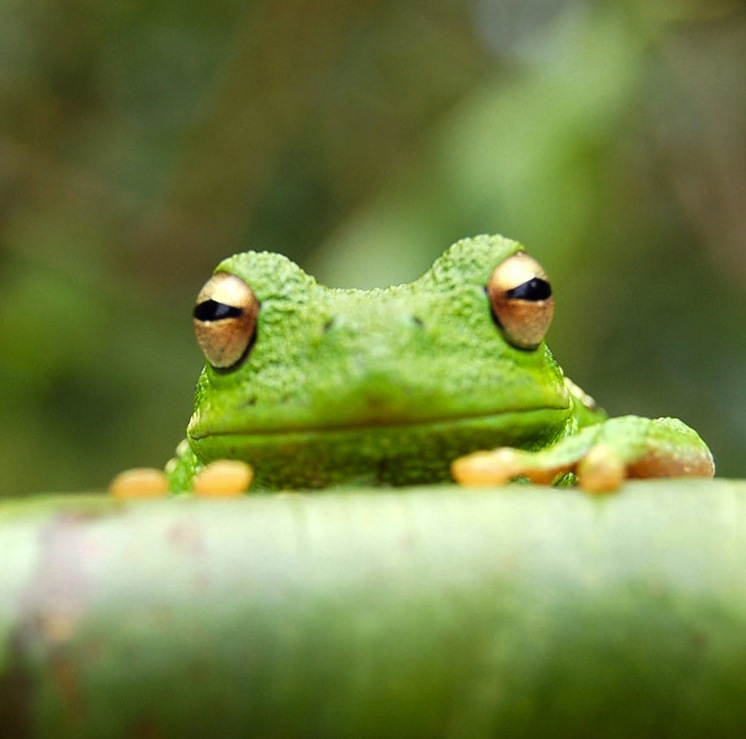
\includegraphics[width=0.5\textwidth]{frog.jpg}
\caption{\label{fig:frog}This is a figure caption.}
\end{figure}

\begin{table}
\centering
\begin{tabular}{l|r}
Item & Quantity \\\hline
Widgets & 42 \\
Gadgets & 13
\end{tabular}
\caption{\label{tab:widgets}An example table.}
\end{table}

\subsection{Mathematics}

\LaTeX{} is great at typesetting mathematics. Let $X_1, X_2, \ldots, X_n$ be a sequence of independent and identically distributed random variables with $\text{E}[X_i] = \mu$ and $\text{Var}[X_i] = \sigma^2 < \infty$, and let
$$S_n = \frac{X_1 + X_2 + \cdots + X_n}{n}
      = \frac{1}{n}\sum_{i}^{n} X_i$$
denote their mean. Then as $n$ approaches infinity, the random variables $\sqrt{n}(S_n - \mu)$ converge in distribution to a normal $\mathcal{N}(0, \sigma^2)$.

\subsection{Lists}

You can make lists with automatic numbering \dots

\begin{enumerate}
\item Like this,
\item and like this.
\end{enumerate}
\dots or bullet points \dots
\begin{itemize}
\item Like this,
\item and like this.
\end{itemize}

We hope you find write\LaTeX\ useful, and please let us know if you have any feedback using the help menu above.

\end{document} to your LaTeX file where you want your
% title page.
%
%%%%%%%%%%%%%%%%%%%%%%%%%%%%%%%%%%%%%%%%%
%\title{Title page with logo}
%----------------------------------------------------------------------------------------
%	PACKAGES AND OTHER DOCUMENT CONFIGURATIONS
%----------------------------------------------------------------------------------------

\documentclass[12pt]{article}
\usepackage[english]{babel}
\usepackage[utf8x]{inputenc}
\usepackage{amsmath}
\usepackage{graphicx}
\usepackage{listings}
\usepackage[colorinlistoftodos]{todonotes}
\usepackage{listings} 
\usepackage{multirow}
\usepackage{booktabs}


\begin{document}

\begin{titlepage}

\newcommand{\HRule}{\rule{\linewidth}{0.5mm}} % Defines a new command for the horizontal lines, change thickness here

\center % Center everything on the page
 
%----------------------------------------------------------------------------------------
%	HEADING SECTIONS
%----------------------------------------------------------------------------------------

\textsc{\LARGE Politenico di Milano}\\[1.5cm] % Name of your university/college
\textsc{\Large Dipartimento Elettronica, Informazione e Bioingegneria}\\[0.5cm] % Major heading such as course name
\textsc{\large HEAPLab Project Report}\\[0.5cm] % Minor heading such as course title

%----------------------------------------------------------------------------------------
%	TITLE SECTION
%----------------------------------------------------------------------------------------

\HRule \\[0.4cm]
{ \huge \bfseries Performance Estimation for TAFFO via LLVM-MCA}\\[0.4cm] % Title of your document
\HRule \\[1.5cm]
 
%----------------------------------------------------------------------------------------
%	AUTHOR SECTION
%----------------------------------------------------------------------------------------

\begin{minipage}{0.4\textwidth}
\begin{flushleft} \large
\emph{Author:}\\
Marco \textsc{Prosdocimi} % Your name
\end{flushleft}
\end{minipage}
~
\begin{minipage}{0.4\textwidth}
\begin{flushright} \large
\emph{Supervisors:} \\
Stefano \textsc{Cherubin} % Supervisor's Name
Daniele \textsc{Cattaneo} % Supervisor's Name
\end{flushright}
\end{minipage}\\[2cm]

% If you don't want a supervisor, uncomment the two lines below and remove the section above
%\Large \emph{Author:}\\
%John \textsc{Smith}\\[3cm] % Your name

%----------------------------------------------------------------------------------------
%	DATE SECTION
%----------------------------------------------------------------------------------------

{\large \today}\\[2cm] % Date, change the \today to a set date if you want to be precise

%----------------------------------------------------------------------------------------
%	LOGO SECTION
%----------------------------------------------------------------------------------------


\includegraphics[width=100pt]{heaplogo.pdf}\\[1cm] % Include a department/university logo - this will require the graphicx package
 
%----------------------------------------------------------------------------------------

\vfill % Fill the rest of the page with whitespace

\end{titlepage}




\begin{abstract}

Use LLVM-MCA to compare the fixed-point code produced by TAFFO with the original floating-point code for all loops in the code. 
LLVM-MCA is a tool that simulates the inner behavior of the CPU to estimate the performance of a machine code snippet.
TAFFO is an autotuning framework, based on LLVM 8, which tries to replace floating-point operations with fixed-point operations as much as possible.

\end{abstract}

\section{Introduction}

The purpose of the project is to write a tool to find body loops in a c program, compile them with and without TAFFO, and use LLVM-MCA checks if TAFFO improves the execution of the loops by reducing the total amount of machine cycles required.

\section{Design and Implementation}
The tool is divided into two different parts: the Loops Finder and the LLVM-MCA analysis.

\subsection{Loop Extractor}
By using the LLVM API, i was able to write an LLVM Pass that searches loops in code and add an Assembly inline comment in the header and the exit block.\\
The Assembly comments are "LLVM-MCA-BEGIN" and "LLVM-MCA-END". They are used in the LLVM-MCA analysis.
In the event of nested loops, the pass marks only the most inner one.\\
Before running this pass, we use the loop simplify pass to try to have simple form loops, with a pre-header and just one exit block.\\
Unfortunately, I'm not always able to render loops with a single exit block in this version of the tool this kind of loops are skipped.\\
OTP executes the Loop Finder Pass after the TAFFO ones.\\

\subsection{LLVM-MCA analysis}

I had to modify the main of LLV-MCA so that he shows the total machine cycle count for all marked regions. LLVM-MCA is designed to print several different analysis concerned the different region that was marked in the code. For this project, I was interested only in the total amount of machine cycle for all the regions.
In the file "llvm-mca-mod.c" I underline the originally LLVM-MCA code and the few lines that I change.


\subsection{Tool Steps}
The tool follows thees main step:
\begin{enumerate}
\item By using CLANG, it compiles the code and emits the LLVM IR.
\item To generate the TAFFO IR file, OPT runs all TAFFO passes, and then the Loop Extractor pass.
\item For the non TAFFO IR file, it executes only Loop Extractor pass.
\item The two IR files are compiled using LLC.
\item Uses the mod version of MCA on both the assembly.
\item Print the results of the analysis for each of the two assembly file.
\end{enumerate}

\section{Experimental Results}
I run the tool on several tests get the MCA analysis for AMD A8-6600K a x86 CPU 64 bit.

\subsection{Polybench benchmarks}
The Polybench benchmarks are 30 different tests that have one loop that dominates all the execution times.
I wrote a shell script that runs those tests with and without TAFFO and use my tools to estimate the number of machine cycles.

\begin{table}[ht]
\begin{center}
\caption{summary of Polybench benchmarks}
\vspace{0.5cm}
\begin{tabular}{ |p{7cm} | p{4cm} | }
 \hline
 \multicolumn{2}{|c|}{Result of LLVM-MCA} \\
 \hline
  Total number of tests improved by TAFFO & 11  \\
  \hline
  Average of machine cycle reduced by TAFFO & 1130 \\
  \hline
\end{tabular}
\end{center}
\end{table}

See Appendix A for more detail about sinlgle tests.
\subsection{Axbench benchmarks}

For these tests, instead of using the shell script tool, i wrote a Make file that compiles the code with and without TAFFO. 
I generating two different assembly code.
Then i use the LLVM-MCA to estimate the machine cycles.

\begin{table}[ht]
\begin{center}
\caption{machine cycle measured by use LLVM MCA for Axbench benchmarks}
\vspace{0.5cm}
\begin{tabular}{ |c|c|c| } 
 \hline
Test Name & Total number of CC & Total number of CC with TAFFO \\
 \hline
  Blackscholes & 6402 & 8571 \\
 \hline
  fft & 36718 & 11281 \\
 \hline
  jmeint & 1720 & 1521 \\
 \hline
  sobel & 27094 & 11149 \\
 \hline
  inversek2j & 102512 & 44571 \\
 \hline
 \end{tabular}
\end{center}
\end{table}

\section{Conclusions and future study}

The tool created is useful in the development of TAFFO but certainly needs some improvements.
The challenging management of some loops makes the tool not entirely usable. In the future, we will have to change the "Loop Extractor" LLVM pass to be able to manage those loops that do not have a single exit block.
This problem is present in some Axebench, so not all tests are fully reliable yet.
In order to see the best TAFFO improvement, it is necessary to do some tests with machines without FPU (Floating point unit). Repeat Axbench and Polybench benchmarks in this machine type can be a useful study.

\newpage
\begin{table}[ht]
\section{\fontsize{12}{15}\selectfont Appendix A Polybenc benchmarks}
\begin{center}
\begin{tabular}{ |c|c|c| } 
 \hline
Test Name & Total number of CC & Total number of CC with TAFFO \\
 \hline
 correlation.c & 11379 & 12851 \\
 \hline
  covariance.c & 7086 & 7910 \\
 \hline
  2mm.c & 18940 & 16261 \\
 \hline
  3mm.c & 20772 & 17490 \\
 \hline
  atax.c & 8660 & 8791 \\
 \hline
  bicg.c & 14088 & 13855 \\
 \hline
  doitgen.c & 11557 & 14282 \\
 \hline
  mvt.c & 10634 & 11150 \\
 \hline
  gemm.c & 13633 & 12105 \\
 \hline
  gemver.c & 10101 & 9892 \\
 \hline
  gesummv.c & 10776 & 9467 \\
 \hline
  symm.c & 12764 & 13384 \\
 \hline
  syr2k.c & 13609 & 12082 \\
 \hline
  syrk.c & 10509 & 9582 \\
 \hline
  trmm.c & 7641 & 7458 \\
 \hline
  cholesky.c & 10705 & 10425 \\
 \hline
  durbin.c & 4789 & 6089 \\
 \hline
  gramschmidt.c & 11949 & 12399 \\
 \hline
  lu.c & 10705 & 10425 \\
 \hline
  ludcmp.c & 13660 & 15862 \\
 \hline
  trisolv.c & 4884 & 5688 \\
 \hline
  deriche.c & 14938 & 22465 \\
 \hline
  floyd-warshall.c & 16627 & 17054 \\
 \hline
  nussinov.c & 8506 & 9807 \\
 \hline
  adi.c & 7968 & 8615 \\
 \hline
  fdtd-2d.c & 13527 & 15870 \\
 \hline
  heat-3d.c & 14331 & 15655 \\
 \hline
  jacobi-1d.c & 5874 & 6283 \\
 \hline
  jacobi-2d.c & 7883 & 8562 \\
 \hline
  seidel-2d.c & 8700 & 9811 \\
 \hline
 
 
\end{tabular}
\end{center}
\end{table}

\end{document}